% !TEX root = ../discretemath.tex

\section{Круговые многочлены}

\subsection{Определение и первые свойства}

\begin{Definition}{Круговой многочлен}{}
	Для натурального $n$:
	\[
	\Phi_n(x)=\!\!\!\prod_{\substack{z\in\mathbb C,\ z^n=1,\\ z^d\neq 1\ \forall\,0<d<n}}\!\!\!(x-z)\in\mathbb C[x],
	\]
	произведение по всем примитивным корням степени $n$ из единицы (тем $z$, для которых $\operatorname{ord}(z)=n$).
\end{Definition}

\begin{Remark}{}{}
	На единичной окружности $\bar z=z^{-1}$; если $z$ — примитивный корень порядка $n$, то и $\bar z=z^{-1}$ тоже. Значит, корни разбиваются на сопряжённые пары и коэффициенты вещественны: $\Phi_n(x)\in\mathbb R[x]$. Целочисленность $\Phi_n(x)\in\mathbb Z[x]$ доказана ниже.
\end{Remark}

Первые круговые многочлены:
\[
\Phi_1(x)=x-1,\quad \Phi_2(x)=x+1,\quad \Phi_3(x)=x^2+x+1,\quad \Phi_4(x)=x^2+1.
\]

\begin{figure}[H]
	\centering
	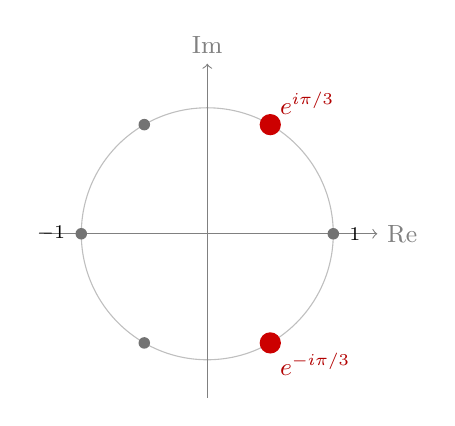
\begin{tikzpicture}[scale=1.6, font=\small]
		\draw[gray!50] (0,0) circle (1);
		\draw[->, gray] (-1.3,0)--(1.35,0) node[right]{$\mathrm{Re}$};
		\draw[->, gray] (0,-1.3)--(0,1.35) node[above]{$\mathrm{Im}$};
		% 6-е корни из единицы
		\foreach \k in {0,1,2,3,4,5}{
			\coordinate (p\k) at ({60*\k}:1);
		}
		% непримитивные (k=0,2,3,4): малые серые
		\foreach \k in {0,2,3,4}{ \fill[black!55] (p\k) circle (1.3pt); }
		% примитивные 6-го порядка: k=1 (60), k=5 (300) — крупные красные
		\fill[red!80!black] (p1) circle (2.4pt);
		\fill[red!80!black] (p5) circle (2.4pt);
		\node[red!70!black, above right] at (p1) {$e^{i\pi/3}$};
		\node[red!70!black, below right] at (p5) {$e^{-i\pi/3}$};
		\node[anchor=west] at (1.05,0) {\scriptsize $1$};
		\node[anchor=east] at (-1.05,0) {\scriptsize $-1$};
	\end{tikzpicture}
	\caption{Корни $6$-й степени из единицы. Примитивные (порядка ровно $6$) выделены красным: их $\varphi(6)=2$, и $\Phi_6(x)=(x-e^{i\pi/3})(x-e^{-i\pi/3})=x^2-x+1$. Остальные корни — примитивные меньших порядков ($1,2,3$) и входят в $\Phi_1,\Phi_2,\Phi_3$.}
\end{figure}

\subsection{Степень кругового многочлена}

Примитивные корни имеют вид $e^{2\pi i k/n}$, $\gcd(k,n)=1$, $0<k\le n$; их ровно $\varphi(n)$.

\begin{Statement}{}{}
	$\deg\Phi_n(x)=\varphi(n)$.
\end{Statement}

\subsection{Разложение $x^n-1$ на круговые многочлены}

\begin{Statement}{}{}
	$\Phi_n(x)\mid(x^n-1)$ — все корни $\Phi_n$ являются корнями $x^n-1$.
\end{Statement}

\begin{Theorem}{}{prod}
	Для любого $n$:
	\[
	x^n-1=\prod_{d\mid n}\Phi_d(x).
	\]
\end{Theorem}

\begin{proof}
	Индукция по $n$. \textbf{База} ($n=1$): $x-1=\Phi_1(x)$.

	\textbf{Переход.} Каждый из $n$ корней $x^n-1$ имеет некоторый порядок $d\mid n$ и попадает ровно в один множитель $\Phi_d(x)$ (по определению примитивности). Оба многочлена — унитарные одной степени $n$ с одинаковым набором корней, поэтому совпадают.
\end{proof}

\subsection{Целочисленность коэффициентов}

\begin{Theorem}{}{}
	$\Phi_n(x)\in\mathbb Z[x]$ для всех $n$.
\end{Theorem}

\begin{proof}
	Индукция по $n$; при $n=1$ — очевидно. Для шага из теоремы~\ref{thm:prod}: $x^n-1=f(x)\cdot\Phi_n(x)$, где $f(x)=\prod_{d\mid n,\,d<n}\Phi_d(x)\in\mathbb Z[x]$ (унитарный) по ИП. Предположим противное: $\Phi_n(x)\notin\mathbb Z[x]$, и пусть $k$ — наибольшая степень с нецелым коэффициентом $\lambda$ (все старшие — целые). Степень $f$ равна $n-\varphi(n)$. В коэффициенте при $x^{n-\varphi(n)+k}$ произведения $f\cdot\Phi_n$ лидирующий член $f$ (равный $1$) умножается на $\lambda$, давая нецелое $\lambda$; все прочие вклады — целые (коэффициенты $\Phi_n$ степени $>k$ целые, $f$ целочислен). Значит, коэффициент при $x^{n-\varphi(n)+k}$ в $f\cdot\Phi_n=x^n-1$ нецелый — противоречие.
\end{proof}

\subsection{Тождество $\Phi_{dn}(x)=\Phi_n(x^d)$}

\begin{Statement}{}{}
	Если $d\mid n$, то $\Phi_{dn}(x)=\Phi_n(x^d)$.
\end{Statement}

\begin{proof}
	\begin{enumerate}
		\item \textbf{Степени.} При $d\mid n$: $\varphi(dn)=d\,\varphi(n)=\deg\Phi_n(x^d)$.
		\item \textbf{Корни.} Пусть $z$ — примитивный $dn$-й корень. Тогда $(z^d)^n=1$; если бы $(z^d)^m=1$ при $m<n$, то $z^{dm}=1$ при $dm<dn$ — противоречие. Значит, $\operatorname{ord}(z^d)=n$, то есть $z$ — корень $\Phi_n(x^d)$.
		\item Оба унитарны одной степени $d\,\varphi(n)$ с одинаковыми корнями, значит равны.
	\end{enumerate}
\end{proof}

\begin{Corollary}{}{}
	Если $p$ простое и $p\mid n$, то $\Phi_{pn}(x)=\Phi_n(x^p)$.
\end{Corollary}

\subsection{Формула Мёбиуса для $\Phi_n$}

Логарифмируя тождество $x^n-1=\prod_{d\mid n}\Phi_d(x)$:
\[
\log(x^n-1)=\sum_{d\mid n}\log\Phi_d(x),
\]
и применяя формулу обращения Мёбиуса:
\[
\log\Phi_n(x)=\sum_{d\mid n}\mu\!\left(\tfrac{n}{d}\right)\log(x^d-1).
\]

\begin{Statement}{}{}
	\[
	\Phi_n(x)=\prod_{d\mid n}(x^d-1)^{\mu(n/d)}=\prod_{d\mid n}\bigl(x^{n/d}-1\bigr)^{\mu(d)}.
	\]
	При $n>1$ свободный член $\Phi_n(x)$ равен $\pm 1$.
\end{Statement}

\begin{Remark}{}{}
	Формула выражает $\Phi_n$ через одночленные множители $x^d-1$ с показателями $\mu(n/d)\in\{-1,0,1\}$ — прямое применение обращения Мёбиуса к мультипликативному тождеству (логарифм переводит произведение в сумму, к которой применимо обращение).
\end{Remark}
